\textbf{Problem 0: Quadrature}

Over a single interval, the trapezoidal rule is
\begin{align}
    \int_a^b f(x) \dd{x} \approx \frac{b-a}{2} [f(a)-f(b)]
\end{align}

The composite trapezoidal rule is given by
\begin{align}
    \int_a^b f(x) \dd{x} \approx \frac{b-a}{n}
    \left[ \frac{f(a) + f(b)}{2} + \sum_{i=1}^{n-1} f\left( a + \frac{i(b-a)}{n} \right) \right]
\end{align}

\begin{enumerate}[label=(\alph*),leftmargin=*,itemsep=0mm]
    
    \item Prove that the error in approximating $I$ via the composite trapezoidal rule is
    \begin{align*}
        \int_a^b f(x) \dd{x} - \frac{b-a}{n}
        \left[ \frac{f(a) + f(b)}{2} + \sum_{i=1}^{n-1} f\left( a + \frac{i(b-a)}{n} \right) \right]
        = -\frac{(b-a)^3}{12n^2} f''(\eta)
    \end{align*}
    
    for some $\eta \in [a,b]$.
    
    \begin{proof}
        
        We consider one interval in this summation, $[x_i,x_{i+1}]$ and let $c=(x_i+x_{i+1})/2$ be the midpoint of this interval.  Let us perform integration by parts on the following integral:
        \begin{align*}
            \int_{x_i}^{x_{i+1}} (x-c) f'(x) \dd{x}
            &= \left[ (x-c)f(x) - \int f'(x) \dd{x} \right] \\
            &= [(x-c)f(x)]_{x_i}^{x_{i+1}} - f(x_{i+1}) + f(x_i) \\
            &= \frac{x_{i+1}-x_i}{2} f(x_{i+1}) + \frac{x_{i+1}-x_i}{2} f(x_{i})
            - f(x_{i+1}) + f(x_i)
        \end{align*}
        
        The error in the composite trapezoidal rule is
        \begin{align*}
            E = \int_{x_i}^{x_{i+1}} f(x) \dd{x} - \frac{x_{i+1}-x_i}{2}f(c)
        \end{align*}
        
    \end{proof}
    
    \item We implement the composite trapezoidal rule (1) and use it to approximate the following integrals for the number of intervals $n=1,\dots,100$.  We calculate the absolute error between the exact integral and the approximate value.  From Fig. \ref{prj3_qn0bqn1b}a, we see that the order of convergence for (i) $I = \int_2^{10} 3x\dd{x}$ does not exist, as $I$ is exact, (ii) $I = \int_0^{\pi} \sin(x) \dd{x}$ is $\mathcal{O}(1/n^2)$, (iii) $\int_0^1 e^{2\cos(2\pi x)} \dd{x}$ is spectral, and (iv) $\int_0^{2\pi} \abs{\cos(x)} \dd{x}$ is $\mathcal{O}(1/n^2)$.

    \begin{figure*}[h!]
    \centering
    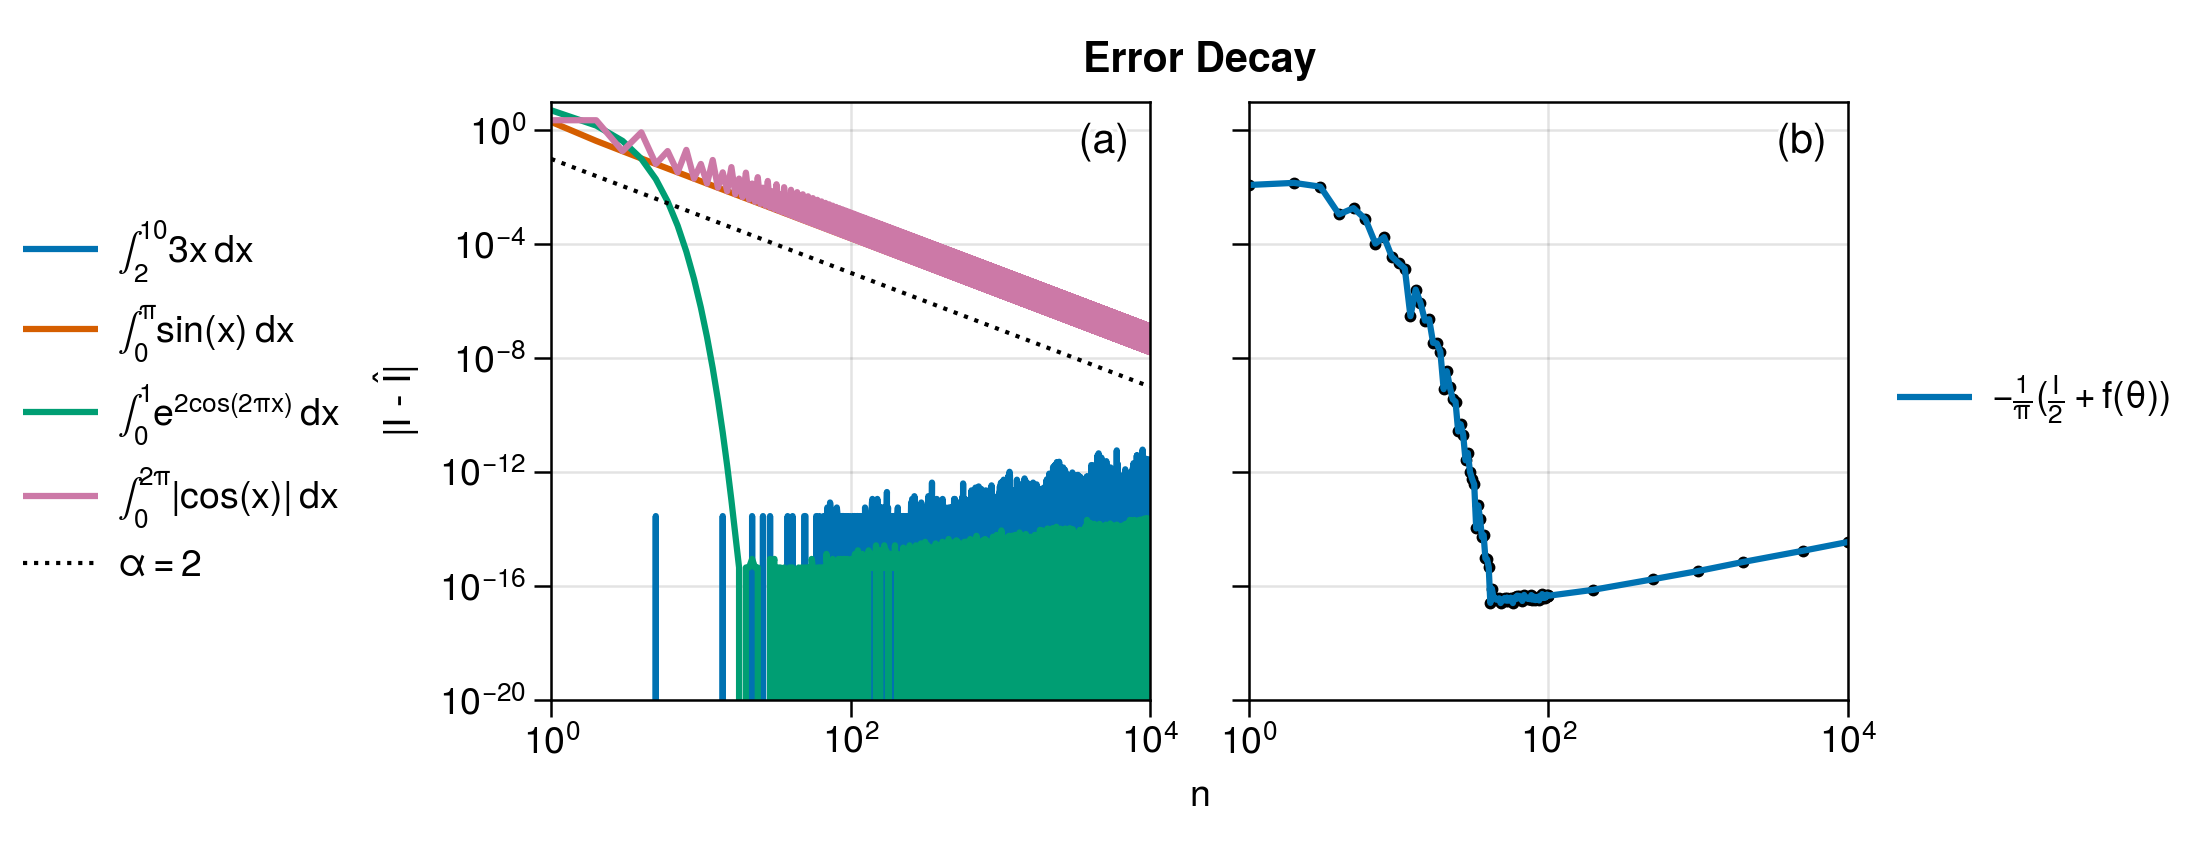
\includegraphics[width=\textwidth]{figures/prj3_qn0bqn1b.png}\\
    \caption{}
    \label{prj3_qn0bqn1b}
    \end{figure*}
    
\end{enumerate}